\documentclass{article}
\usepackage{ifthen}
\usepackage{amssymb}
\usepackage{multicol}
\usepackage{graphicx}
\usepackage[absolute]{textpos}
\usepackage{amsmath, amscd, amssymb, amsthm, latexsym}
\usepackage{xspace,rotating,dsfont,ifthen}
\usepackage[spanish,activeacute]{babel}
\usepackage[utf8]{inputenc}
\usepackage{pgfpages}
\usepackage{pgf,pgfarrows,pgfnodes,pgfautomata,pgfheaps,xspace,dsfont}
\usepackage{listings}
\usepackage{multicol}
\usepackage{todonotes}
\usepackage{url}
\usepackage{float}
\usepackage{framed,mdframed}
\usepackage{cancel}

\usepackage[strict]{changepage}


\makeatletter


\newcommand\hfrac[2]{\genfrac{}{}{0pt}{}{#1}{#2}} %\hfrac{}{} es un \frac sin la linea del medio

\newcommand\Wider[2][3em]{% \Wider[3em]{} reduce los m\'argenes
\makebox[\linewidth][c]{%
  \begin{minipage}{\dimexpr\textwidth+#1\relax}
  \raggedright#2
  \end{minipage}%
  }%
}


\@ifclassloaded{beamer}{%
  \newcommand{\tocarEspacios}{%
    \addtolength{\leftskip}{4em}%
    \addtolength{\parindent}{-3em}%
  }%
}
{%
  \usepackage[top=1cm,bottom=2cm,left=1cm,right=1cm]{geometry}%
  \usepackage{color}%
  \newcommand{\tocarEspacios}{%
    \addtolength{\leftskip}{3em}%
    \setlength{\parindent}{0em}%
  }%
}

\usepackage{caratula}
\usepackage{enumerate}
\usepackage{hyperref}
\usepackage{graphicx}
\usepackage{amsfonts}
\usepackage{enumitem}

\decimalpoint
\hypersetup{colorlinks=true, linkcolor=black, urlcolor=blue}
\setlength{\parindent}{0em}
\setlength{\parskip}{0.5em}
\setcounter{tocdepth}{2} % profundidad de indice
\setcounter{section}{0} % nro de section
\renewcommand{\thesubsubsection}{\thesubsection.\Alph{subsubsection}}
\graphicspath{ {images/} }

% End latex config

\begin{document}

\titulo{Práctica 1}
\fecha{2do cuatrimestre 2021}
\materia{Álgebra I}
\integrante{Yago Pajariño}{546/21}{ypajarino@dc.uba.ar}

%Carátula
\maketitle
\newpage

%Indice
\tableofcontents
\newpage

% Aca empieza lo propio del documento
\section{Práctica 1}

\subsection{Ejercicio 1}
\begin{enumerate}[label=(\alph*)]
    \item Verdadero
    \item Falso
    \item Verdadero
    \item Falso
    \item Falso
\end{enumerate}

\subsection{Ejercicio 2}
\begin{enumerate}[label=(\alph*)]
    \item Falso
    \item Falso
    \item Verdadero
    \item Verdadero
    \item Verdadero
    \item Verdadero
    \item Verdadero
    \item Falso
    \item Falso
    \item Verdadero
    \item Falso
    \item Verdadero
\end{enumerate}

\subsection{Ejercicio 3}
Rdo.: Sean A y B conjuntos. $ A \subseteq B \iff \forall x \in A \rightarrow x \in B$
\begin{enumerate}[label=(\alph*)]
    \item $A \subseteq B$
    \item $A \not \subseteq B$ pues $3 \not \in B$
    \item $A \not \subseteq B$ pues $2.25 \not \in B$
    \item $A \subseteq B$
\end{enumerate}

\subsection{Ejercicio 4}
\begin{enumerate}[label=(\alph*)]
    \item $A \cap (B \triangle C) = \{ 1,-2,3 \}$
    \item $(A \cap B) \triangle (A \cap C) = \{1,-2,3\}$
    \item $A^c \cap B^c \cap C^c = \emptyset$ 
\end{enumerate}

\subsection{Ejercicio 5}
Rdo. DeMorgan: Sean A y B conjuntos, $(A \cap B)^c = (A^c \cup B^c)$ y $(A \cup B)^c = (A^c \cap B^c)$

\begin{enumerate}
    \item $(A \cup B \cup C)^c = A^c \cap B^c \cap C^c$
    \item $(A \cap B \cap C)^c = A^c \cup B^c \cup C^c$
\end{enumerate}

\subsection{Ejercicio 6}
\begin{enumerate}[label=(\alph*)]
    \item 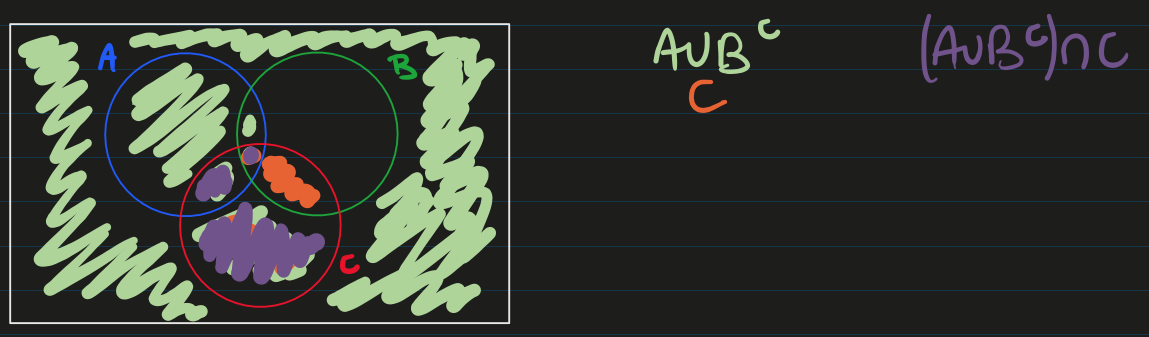
\includegraphics[width=500px]{1.6.1}
    \item 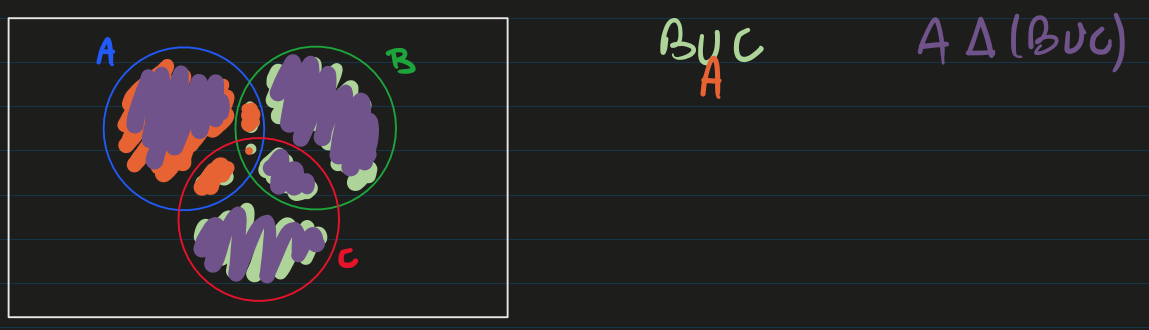
\includegraphics[width=500px]{1.6.2}
    \item 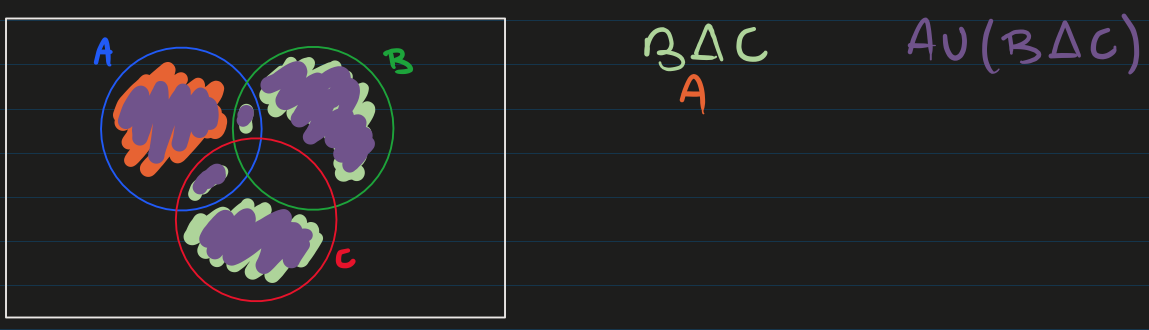
\includegraphics[width=500px]{1.6.3}
\end{enumerate}

\subsection{Ejercicio 7}
\begin{enumerate}[label=(\alph*)]
    \item $(A \cap B^c) \cup (B \cap C \cap A^c)$
    \item $((A \cap C^c) \cup (C \cap A^c)) \cap B^c$
    \item $(A \cap B) \cup (A \cap C) \cup (B \cap C) \cap (A \cap B \cap C)^c$
\end{enumerate}

\subsection{Ejercicio 8}
Rdo. conjunto de partes: Sea A un conjunto, el conjunto de partes de A, $P(A)$ es aquel formado por todos los subonjuntos de A.

\begin{enumerate}[label=(\alph*)]
    \item $P(A) = \{ \emptyset, \{ 1 \} \}$
    \item $P(A) = \{ \emptyset, \{ a \}, \{ b \}, \{ a, b \} \}$
    \item $P(A) = \{ \emptyset, \{ 1 \}, \{ \{ 1,2 \} \}, \{ 3 \}, \{ 1, \{1,2\} \}, \{ 1,3 \}, \{\{1,2\}, 3 \}, \{ 1,\{1,2\}, 3 \} \}$
\end{enumerate}

\subsection{Ejercicio 9}
Quiero probar un $(\iff)$ por lo que debo verificar la doble inclusión.

\begin{enumerate}[label=(\alph*)]
    \item $A \subseteq B \rightarrow P(A) \subseteq P(B)$ 
            Sea x tal que $x \in P(A) \rightarrow (\forall y \in x): y \in A$.\\
            Pero $A \subseteq B \rightarrow y \in B$.
            Por lo tanto $(\forall x \in P(A)): x \in P(B) \rightarrow P(A) \subseteq P(B)$
    \item $P(A) \subseteq P(B) \rightarrow A \subseteq B$ 
            Por definición del conjunto de partes, $A \in P(A)$ por lo tanto se que $A \in P(B)$ \\
            Además $B \in P(B)$ y es el elemento con más elementos de $P(B)$, así $A \subseteq B$ como se quiería probar.
\end{enumerate}

\subsection{Ejercicio 10}

\subsubsection{Inciso a}
Calculadora de tablas de verdad. \href{https://calculadorasonline.com/generador-de-tablas-de-verdad-logica-proposicional-algebra-booleana/}{Link}\\

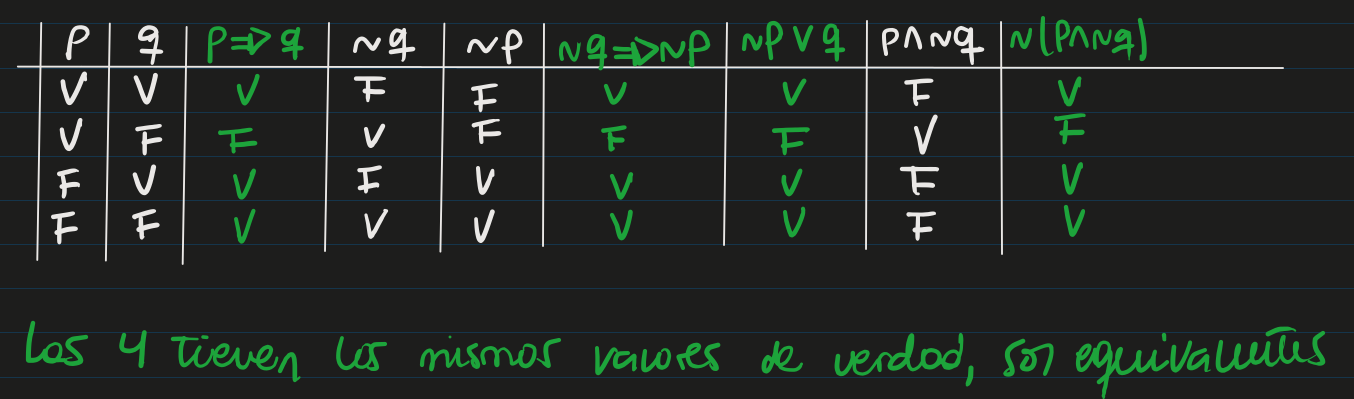
\includegraphics[width=500px]{1.10}

\subsubsection{Inciso b}
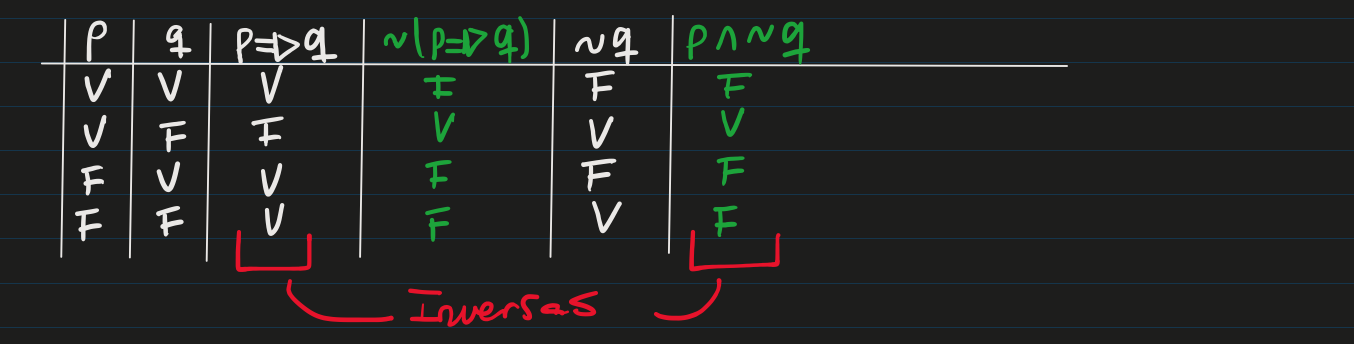
\includegraphics[width=500px]{1.11}

\subsection{Ejercicio 11}
\begin{enumerate}[label=(\alph*)]
    \item $a = 1$ pues $1 \in \mathbb{N}$ pero $\frac{1-1}{1} = 0 \not \in \mathbb{N}$.
    \item $x = y = 4$ pues $\sqrt{4+4} = \sqrt{8} \neq 4 = \sqrt{4} + \sqrt{4}$
    \item $x = -3$ pues $(-3)^2 = 9 > 4$ sin embargo $(-3) \not > 2$
\end{enumerate}

\subsection{Ejercicio 12}
\begin{enumerate}[label=(\alph*)]
    \item El $\vee$ lógico es falso unicamente cuando ambas preposiciones son falsas. Así, la proposición será falsa sii $(x < 5) \wedge (x > 8)$
            Pero es fácil ver que no existe ningún $x \in \mathbb{N}$ que lo cumpla.
    \item Es verdadera pues $n = 6$ hace verdadera la proposición $(n \geq 5) \wedge (n \leq 8)$
    \item Es verdadera pues el conjunto de los $\mathbb{N}$ es infinito y por lo tanto existe $m = n+1$ que hace verdadera la proposición.
    \item Es falsa pues no existe un natural $n$ tal que $1 > n$.
    \item Es verdadera pues $f(x) = x^2$ es una función estrictamente creciente en el intervalo $[0, \infty]$ y dado que $f(3) = 9 > 4$ podemos afirmar que la preposición es verdadera.
    \item Es verdadera pues sea $c \in \mathbb{C} \rightarrow c = a+b.i$ con $a,b \in \mathbb{R}$ y por lo tanto $(\forall r \in \mathbb{R}): (r + 0.i) \in \mathbb{C} $
\end{enumerate}

\subsection{Ejercicio 13}
\begin{enumerate}[label=(\alph*)]
    \item 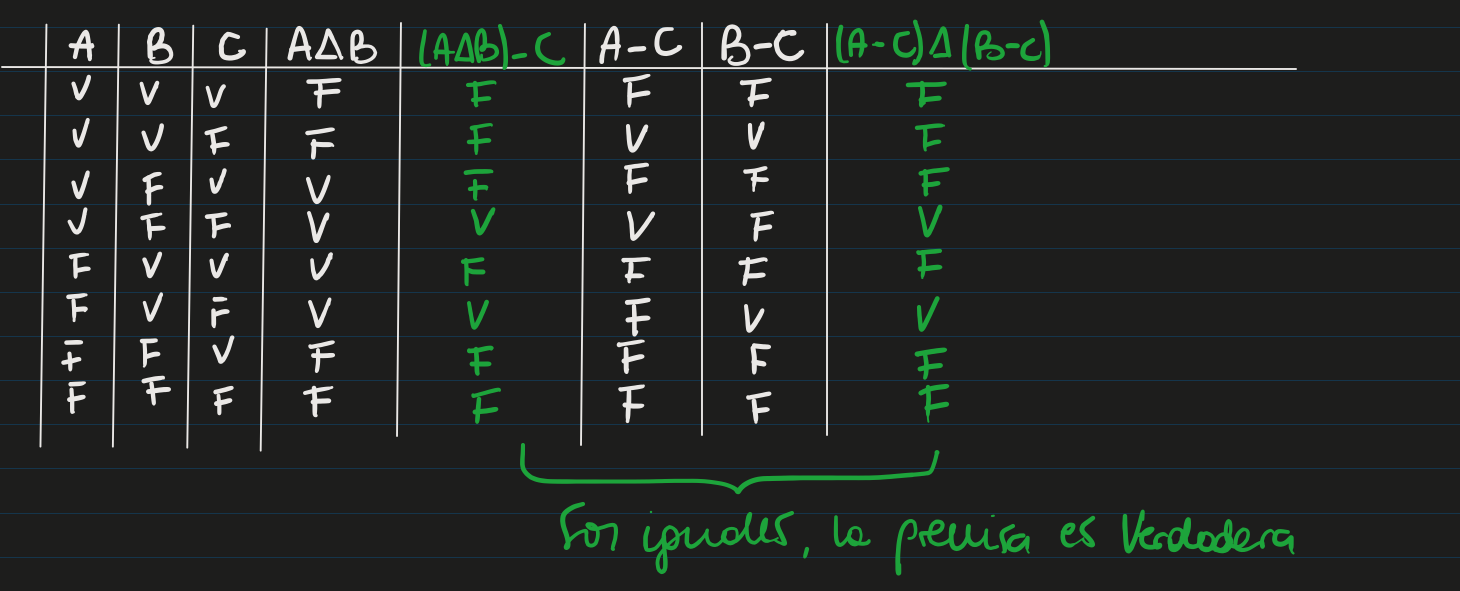
\includegraphics[width=500px]{1.13.1}
    \item Falsa. Contraejemplo. $A=\{1\}$ $B=\{2\}$ $C=\{1\}$ 
    \item 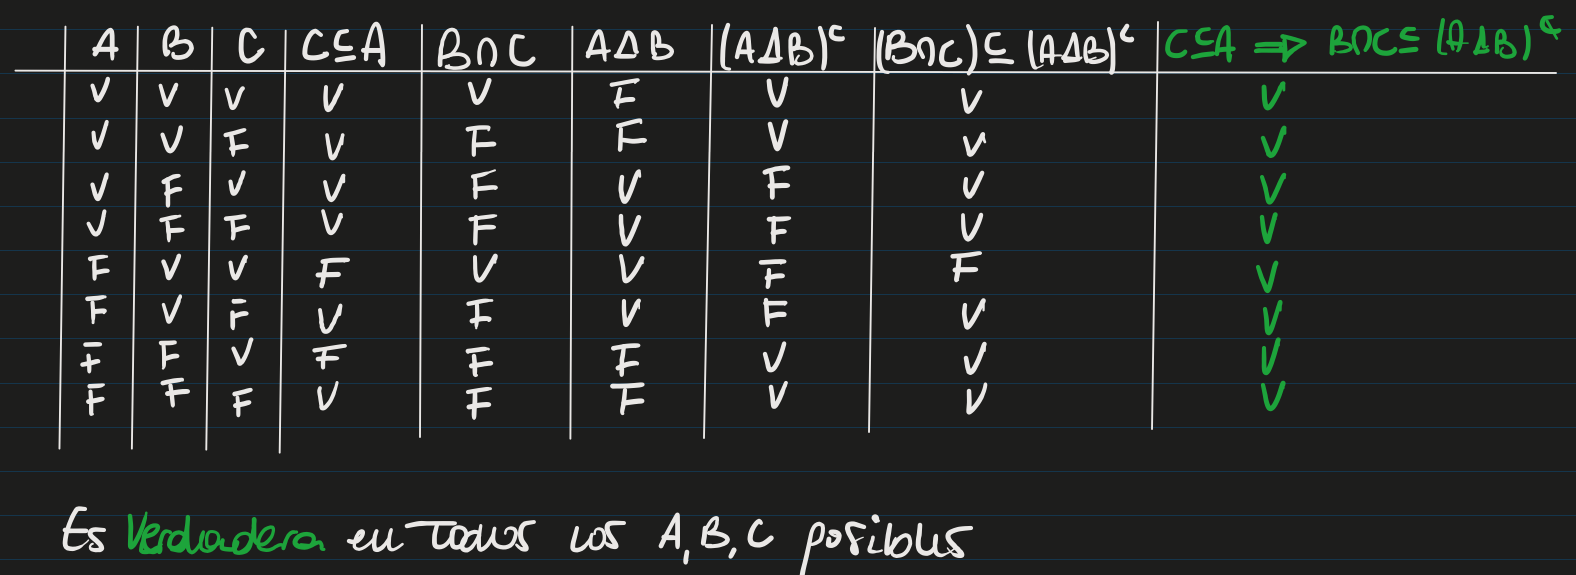
\includegraphics[width=500px]{1.13.3}
    \item 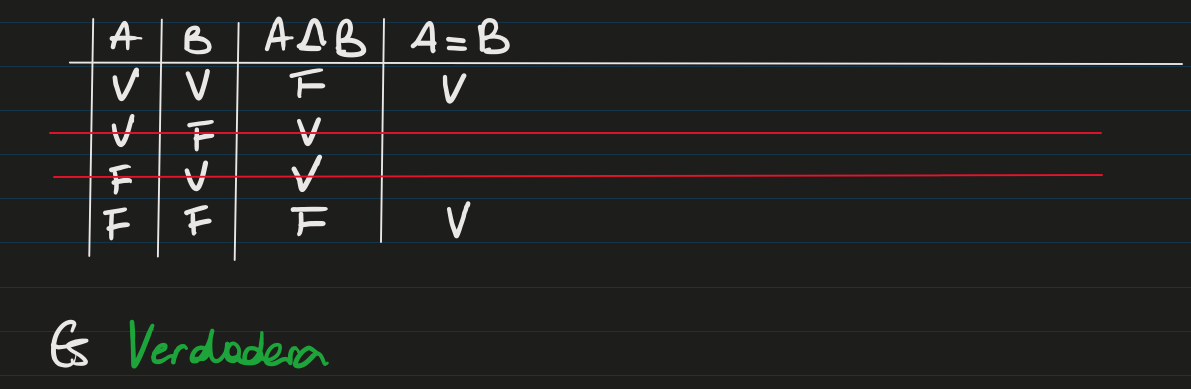
\includegraphics[width=500px]{1.13.4}
\end{enumerate}

\subsection{Ejercicio 14}
Se prueban con tablas de verdad. Van los primeros cuatro.
\begin{enumerate}[label=(\alph*)]
    \item 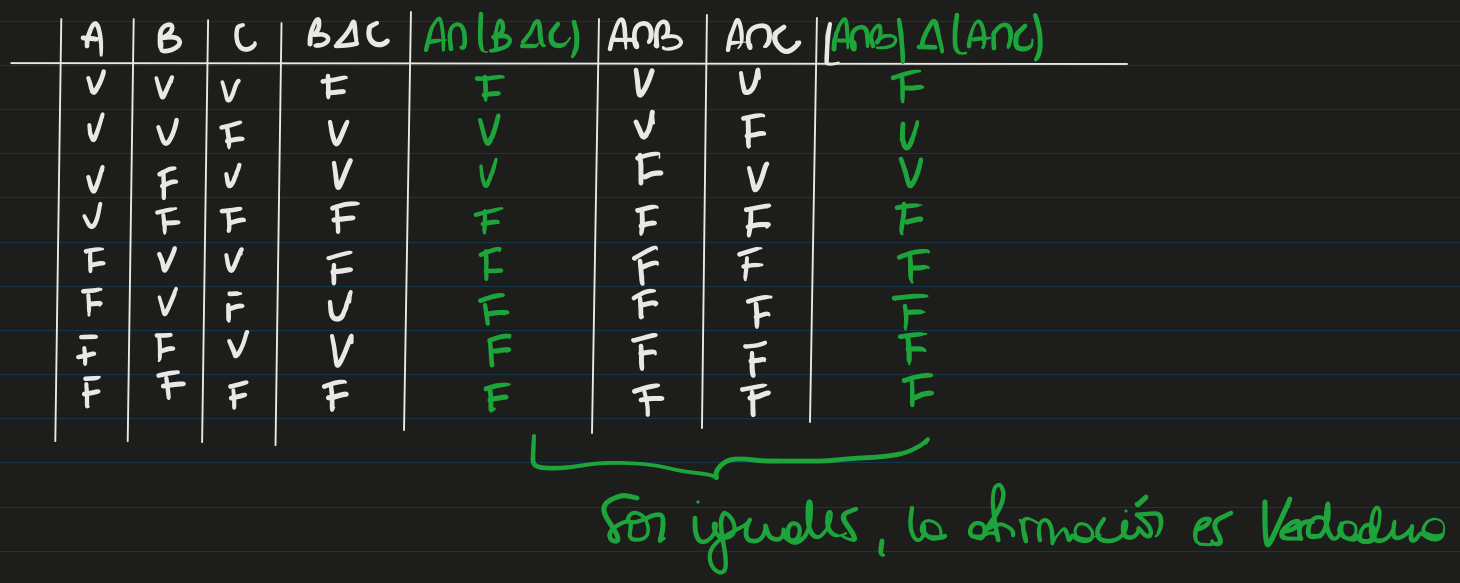
\includegraphics[width=500px]{1.14.1}
    \item 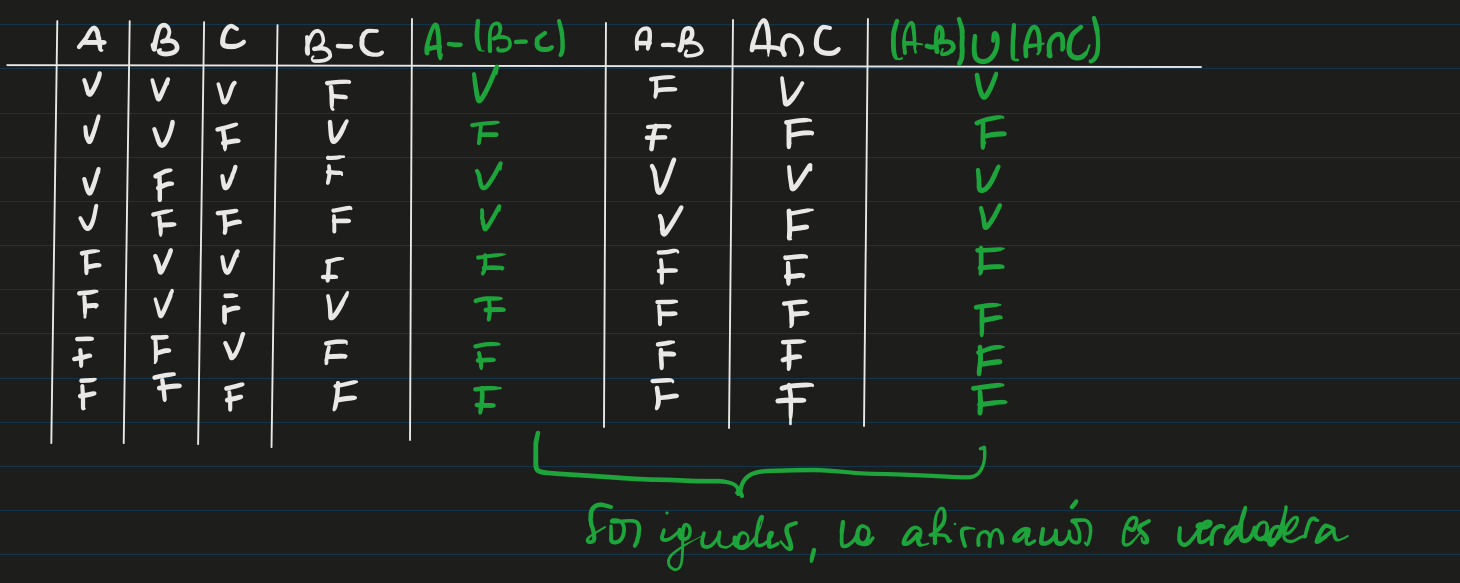
\includegraphics[width=500px]{1.14.2}
    \item 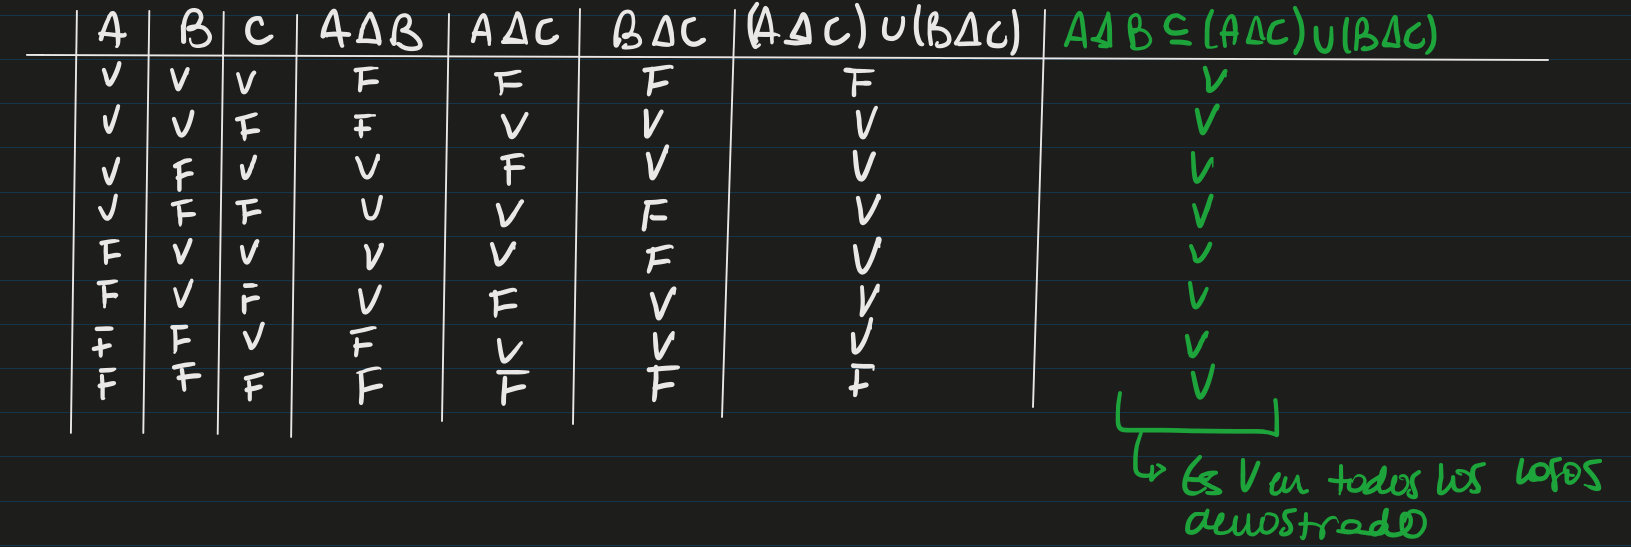
\includegraphics[width=500px]{1.14.3}
    \item 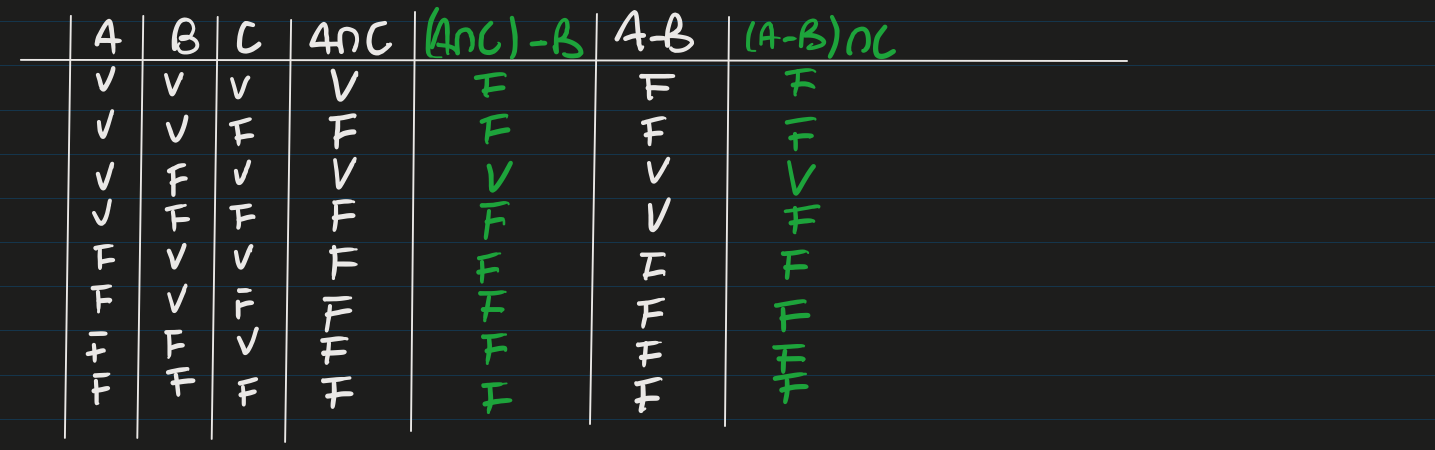
\includegraphics[width=500px]{1.14.4}
    \item TODO
    \item TODO
    \item TODO
\end{enumerate}

\subsection{Ejercicio 15}
\begin{enumerate}
    \item $A \times A = \{(1,1),(1,2),(1,3),(2,1),(2,2),(2,3),(3,1),(3,2),(3,3)\}$
    \item $A \times B = \{(1,1),(1,3),(1,5),(1,7),(2,1),(2,3),(2,5),(2,7),(3,1),(3,3),(3,5),(3,7)\}$
    \item $(A\cap B) \times (A\cup B) = \{(1,1),(1,2),(1,3),(1,5),(1,7),(3,1),(3,2),(3,3),(3,5),(3,7)\}$
\end{enumerate}

\subsection{Ejercicio 16}
Pruebo la doble implicación. 
\begin{enumerate}[label=(\alph*)]
    \item TODO
    \item TODO
    \item \begin{enumerate}
        \item $(A \cup B) \times C \rightarrow (A \times C) \cup (B \times C)$\\
                $(x, y) \in (A\cup B) \times C \iff (x \in (A\cup B) \wedge y \in C) \iff ((x \in A \vee x \in B) \wedge y \in C)$\\
                $\iff (x,y) \in (A\times C) \cup (B \times C)$
        \item $(A \times C) \cup (B \times C) \rightarrow (A \cup B) \times C$\\
                $(x,y) \in (A \times C) \cup (B \times C) \iff ((x \in A \vee x \in B) \wedge y\in C) \rightarrow (x\in (A \cup B) \wedge y \in C)$\\
                $\rightarrow (x, y) \in (A \cup B) \times C$ 
    \item TODO
    \end{enumerate}
\end{enumerate}

\subsection{Ejercicio 17}
Rdo. relación: Sean $A$ y $B$ conjuntos, $R$ es relación de $A$ en $B$ si $R \subseteq A\times B$ es decir, si $R$ es un subonjunto del producto cartesiano $A \times B$\\
$R \subseteq A \times B \iff \forall (X,y) \in R : (x \in A \wedge y \in B)$

\begin{enumerate}[label=(\alph*)]
    \item 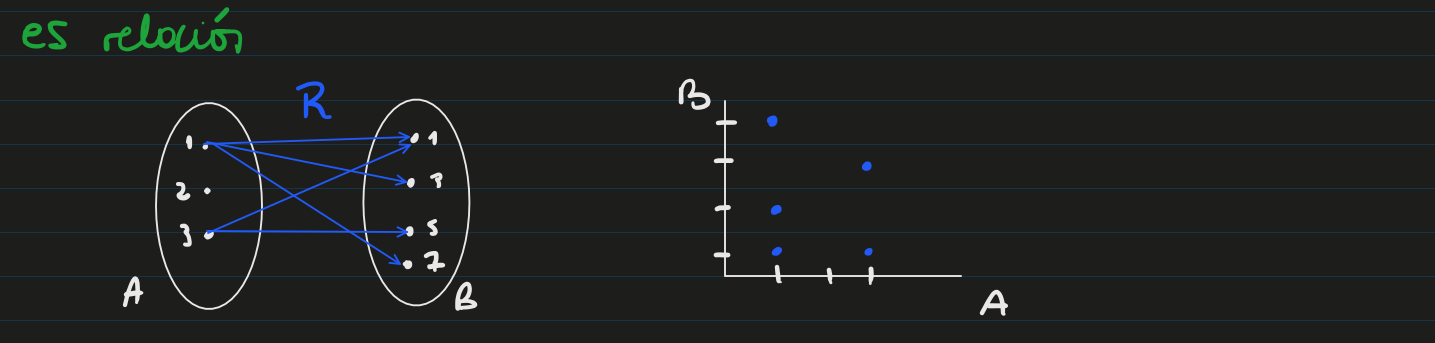
\includegraphics[width=500px]{1.17.1}
    \item No es relación $(3,2) \not \in A\times B$ pues $2 \not \in B$
    \item 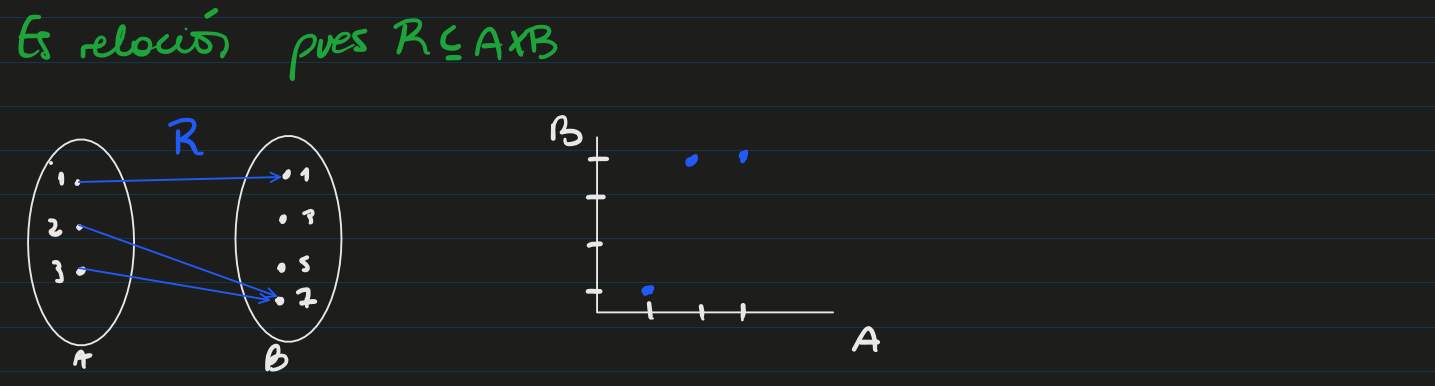
\includegraphics[width=500px]{1.17.3}
    \item 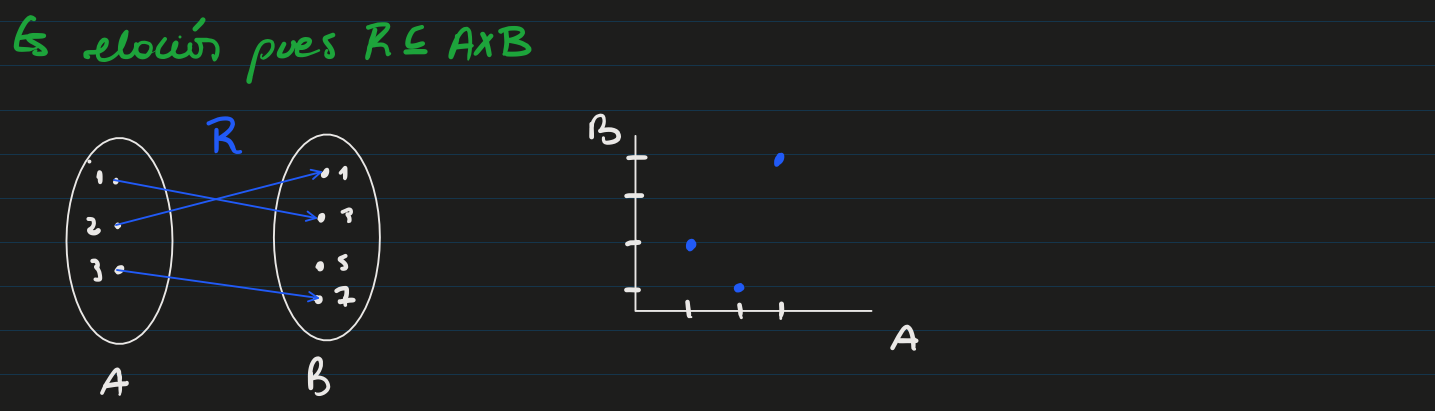
\includegraphics[width=500px]{1.17.4}
\end{enumerate}

\subsection{Ejercicio 18}
\begin{enumerate}[label=(\alph*)]
    \item $R = \{ (1,1), (1,3), (1,5), (1,7), (2,3), (2,5), (2,7), (3,3), (3,5), (3,7) \}$
    \item $R = \{ (2,1), (3,1) \}$
    \item $R = \{ (2,1), (2,3), (2,5), (2,7) \}$
    \item $R = \{ (1,7), (2,5), (2,7), (3,5), (3,7) \}$
\end{enumerate}

\subsection{Ejercicio 19}
\begin{enumerate}[label=(\alph*)]
    \item NO es reflexiva, simétrica, antisimétrica, transitiva.\\
        $R = \{ (a,b), (b,a), (c,c), (c,d), (c,h), (e,c), (f,f), (h,g) \}$
    \item ES transitiva. NO es reflexiva, simétrica, antisimétrica.\\ 
        $R = \{ (a,a), (a,b), (b,b), (b,a), (c,c), (c,e), (c,h), (c,g), (f,f), (h,g) \}$
    \item ES reflexiva. NO es simétrica, antisimétrica, transitiva.\\
        $R = \{ (a,a), (a,b), (b,a), (b,b), (c,c), (c,d), (c,e), (c,h), (d,c), (d,d), (e,e), (f,f), (g,g), (h,h), (h,g) \}$
    \item Es reflexiva, simétrica y transitiva. NO es antisimétrica. \\
        $R = \{ (a,a), (a,b), (b,a), (b,b), (c,c), (d,d), (e,e), (e,h), (e,g), (f,f), (g,e), (g,g), (g,h), (h,h), (h,e), (h,g) \}$ 
\end{enumerate}

\subsection{Ejercicio 20}
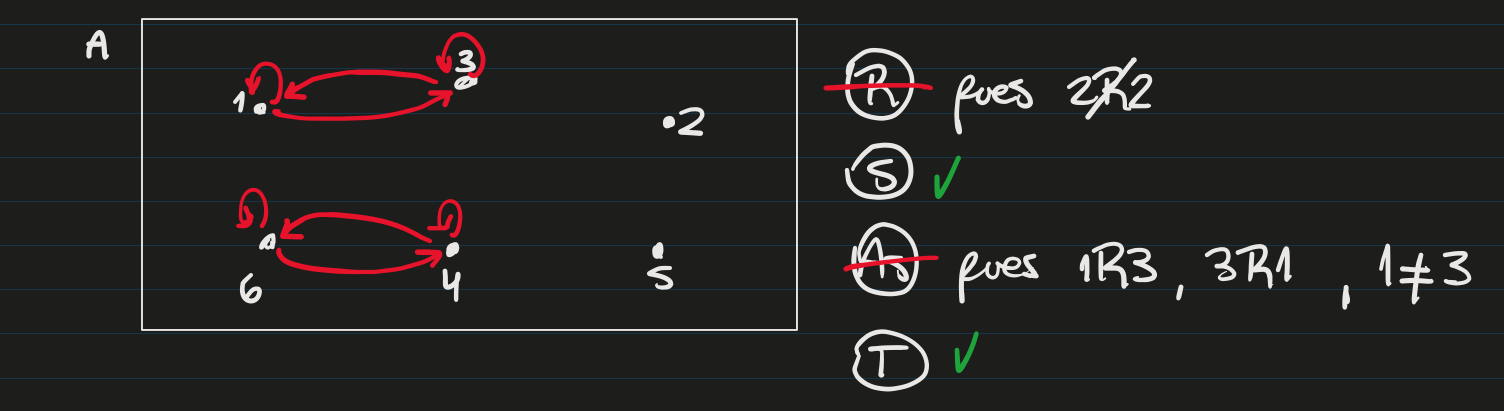
\includegraphics[width=500px]{1.20}

\subsection{Ejercicio 21}
\begin{enumerate}[label=(\alph*)]
    \item 4 pares.
    \item 1 pares.
    \item 1 pares.
    \item 5 pares.
    \item 4 pares.
    \item 5 pares.
\end{enumerate}

\subsection{Ejercicio 22}
\begin{enumerate}[label=(\alph*)]
    \item Es relación de orden.
    \item Es relación de equivalencia.
    \item Es relación de orden.
    \item Es reflexiva y transitiva.
\end{enumerate}

\subsection{Ejercicio 23}
\begin{enumerate}[label=(\alph*)]
    \item Una relación es simétrica sii $(a,b) \rightarrow (b,a) \in \mathbb{R}$ \\
        Una relación es antisimétrica sii $((a,b) \in \mathbb{R} \wedge (b,a) \in \mathbb{R}) \rightarrow a = b$ \\
        Luego, las relaciones en $A$ simétricas y antisimétricas son de la forma: \\
        $R = \{ (a,b) \in A^2 / a = b \}$
    \item R también es de orden y equivalencia, pues es reflexiva y transitiva.
\end{enumerate}

La relación $R = \emptyset$ no es simétrica ni antisimétrica.

\subsection{Ejercicio 24}
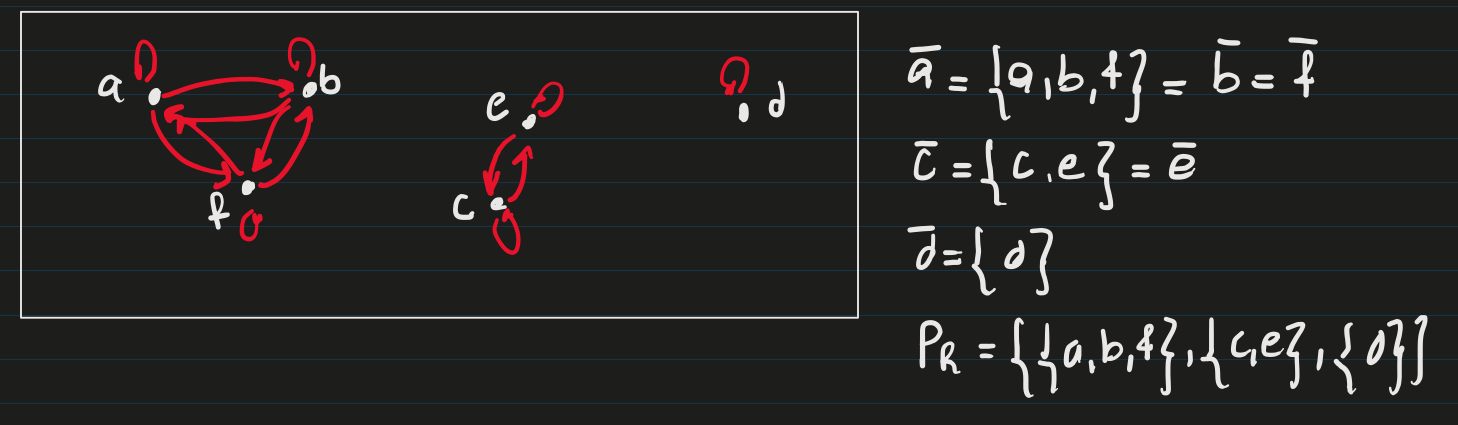
\includegraphics[width=500px]{1.24}

\subsection{Ejercicio 25}
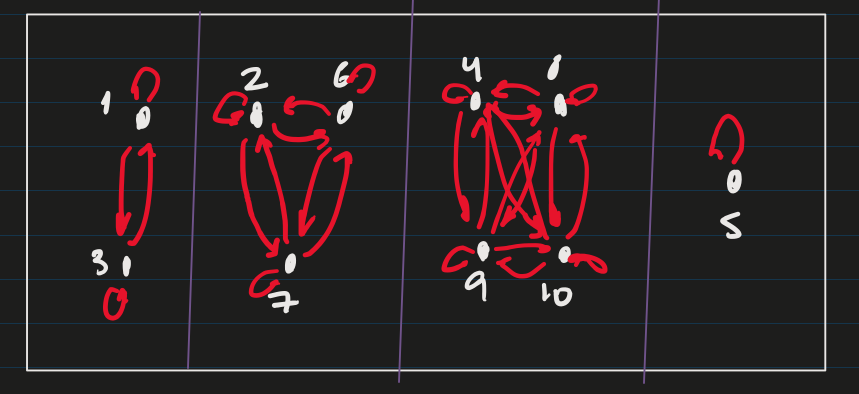
\includegraphics[width=500px]{1.25}

Tiene cuatro clases de equivalencia. Representantes: $\tilde{1} = 1; \tilde{2} = 2; \tilde{4} = 4; \tilde{5} = 5$

\subsection{Ejercicio 26}
Demostración de relación de equivalencia. Vamos a probar que es reflexiva y simétrica y transitiva, cada uno por separado.

\underline{Reflexividad}

$R$ es reflexiva sii A$R$A \\
Por definición, $ARA \iff ((A \triangle A) \cap \{ 1,2,3 \} = \emptyset) $\\
Por definición de la diferencia simétrica, $(A \triangle A) = \emptyset$ \\
Por lo tanto, $\emptyset \cap \{ 1,2,3 \} = \emptyset$ como se quería probar.

Así, $R$ es \textbf{reflexiva}.

\underline{Simetría}

$R$ es simétrica $\iff ARA \rightarrow BRA$.\\
Por definición, $ARB \iff (A \triangle B) \cap \{ 1,2,3 \} = \emptyset$ \\
Por definición de la diferencia simétrica, $(A \triangle B) = (B \triangle A)$ \\
Por lo tanto, $(A \triangle B) \cap \{ 1,2,3 \} = (B \triangle A) \cap \{ 1,2,3 \}$
Y por definición se que $(B \triangle A) \cap \{ 1,2,3 \} \iff BRA$ como se quería probar.

Así, $R$ es \textbf{simétrica}.

\underline{Transitividad}

$R$ es transitiva $\iff (ARB \wedge BRC \rightarrow ARC)$.\\
Por definición, \\$ARB \iff (A \triangle B) \cap \{ 1,2,3 \} = \emptyset$ \\
                  $BRC \iff (B \triangle C) \cap \{ 1,2,3 \} = \emptyset$ \\
                  $ARC \iff (A \triangle C) \cap \{ 1,2,3 \} = \emptyset$

Por ejercicio 14.3, $(A \triangle B) \subseteq (A \triangle B) \cup (B \triangle C)$

Por lo tanto, $ARC \iff ((A \triangle B) \cup (B \triangle C)) \cap \{ 1,2,3 \} = \emptyset$

Haciendo distributiva, $ARC \iff ((A \triangle B) \cap \{ 1,2,3 \}) \cup ((B \triangle C) \cap \{ 1,2,3 \}) = \emptyset$

Pero se que, \\ $(A \triangle B) \cap \{ 1,2,3 \} = \emptyset$ y \\ $(B \triangle C) \cap \{ 1,2,3 \} = \emptyset$

Entonces, $ ARC \iff (\emptyset \cup \emptyset = \emptyset) $ que es verdadero.

Así, $R$ es \textbf{transitiva}.

Dado que $R$ es refelexiva, simétrica y transitiva, queda demostrado que $R$ es una \textbf{relación de equivalencia}.

\underline{Antisimétria}

$R$ es antisimétrica $\iff (ARB \wedge BRA \rightarrow B=A)$.

Contraejemplo: $A = \{ 4 \}$; $B = \emptyset$

$ARB \iff (A \triangle B) \cap \{ 1,2,3 \} = \emptyset$ \\
$ARB \iff \{ 4 \} \cap \{ 1,2,3 \} = \emptyset$ es verdadero.

$BRA \iff (B \triangle A) \cap \{ 1,2,3 \} = \emptyset$ \\
$BRA \iff \{ 4 \} \cap \{ 1,2,3 \} = \emptyset$ es verdadero.

Por lo tanto $ARB$ y $BRA$ pero $A\neq B$

Así, $R$ NO es \textbf{antisimétrica}.

(2) Busco la clase de equivalencia del $\{ 1,2,3 \}$

Se que la clase de equivalencia está formada por todos los $B\in P$ tales que:\\
$\{ 1,2,3 \}RB \iff (\{ 1,2,3 \} \triangle B) \cap \{ 1,2,3 \} = \emptyset$

Por definición de la diferencia simétrica, los $B$ que cumple esto son:

$ \overline{\{ 1,2,3 \}} = \{B \in P / \{ 1,2,3 \} \subset B \}$

\subsection{Ejercicio 27}
(1) De nuevo vamos a probar por separado la refexividad, simetría y transitividad.

\underline{Reflexividad}

$R$ es reflexiva $\iff (\forall x \in A): xRx$

Por definición, $xRx \iff x^2 - x^2 = 93x - 93y \iff 0 = 0$

Así, $R$ es \textbf{reflexiva}.

\underline{Simetría}

$R$ es simétrica $\iff (\forall x, y \in A): xRy \rightarrow yRx$

Por definición, 
\begin{align*}
    xRy &\iff x^2 - y^2 = 93x - 93y \\
    &\iff -x^2 + y^2 = -93x +93y \\
    &\iff y^2 -x^2 = 93y -93x \\
    &\iff yRx
\end{align*}

Así, $R$ es \textbf{simétrica}.

\underline{Transitividad}

$R$ es transitiva $\iff (\forall x, y, z \in A): (xRy \wedge yRz) \rightarrow xRz$

Por definición,
\begin{align*}
    xRy \iff x^2 - y^2 = 93x - 93y \\
    yRz \iff y^2 - z^2 = 93y - 93z
\end{align*}

Sumando ambas,
\begin{align*}
    x^2 - y^2 + y^2 - z^2 &= 93x - 93y +93y - 93z \\
    \iff x^2 -z^2 &= 93x - 93z \iff xRz 
\end{align*}

Así, $R$ es \textbf{transitiva}.

Por lo tanto, $R$ es reflexiva, simétrica y transitiva; luego $R$ es una \textbf{relación de equivalencia}.

(2) $\overline{x} = \{ x, 93-x \}$

\subsection{Ejercicio 28}
Habrá una clase de equivalencia para cada cardinal posible en los subconjuntos de $P(A)$ es decir,
\begin{enumerate}[label=(\alph*)]
    \item $\tilde{1} = \{ \text{subconjuntos con }\#=1 \}$
    \item $\tilde{2} = \{ \text{subconjuntos con }\#=2 \}$
    \item $\tilde{3} = \{ \text{subconjuntos con }\#=3 \}$
    \item etc
\end{enumerate}

Lo que define 10 clases de equivalencia, más la clase $\tilde{0} = \emptyset$ determinan 11 clases de equivalencia.

\subsection{Ejercicio 29}
Rdo. función: Una relación $R \subseteq A\times B$ es una función de A en B si: $\forall x \in A, \exists ! y \in B / xRy$

\begin{enumerate}[label=(\alph*)]
    \item No. El 3 tiene dos asignaciones en R: $(3,a) y (3,d)$
    \item No. El 5 no tiene asignación en R.
    \item Sí
    \item Sí
    \item No. $\not \exists b \in \mathbb{N}: 2b-3 = \pi$
    \item No. Tomando $a = 1$ se obtiene más de un valor en $R: (1,4), (1,9)$
\end{enumerate}

\subsection{Ejercicio 30}

\subsubsection{Inciso 1}

\underline{Inyectiva}

Por definición, f es inyectiva $\iff \forall x, y \in \mathbb{R}: f(x) = f(y) \rightarrow x = y$

Contraejemplo: $x = 1; y=-1$

$f(x) = 12-5 = 7$\\
$f(y) = 12-5 = 7$

Luego $f(x) = f(y)$ pero $x \neq y$

Así, f NO es \textbf{inyectiva}.

\underline{Sobreyectiva}

Por definición, f es sobreyectiva $\iff Im(f) = \mathbb{R}$

Pero por ej. $\not \exists x \in \mathbb{R}: f(x) = -6$ pues $f(x) = 12x^2 -5 \geq -5, \forall x \in \mathbb{R}$

Así, f NO es \textbf{sobreyectiva}.

$Im(f) = \mathbb{R}_{\geq -5}$

\subsubsection{Inciso 2}

\underline{Inyectiva}

Por definición, f es inyectiva $\iff \forall a,b,c,d \in \mathbb{R}: f(a,b) = f(c,d) \rightarrow (a,b) = (c,d)$

Contraejemplo: $(1,3), (2,2)$

$f(1,3) = 1+3 = 4$ \\
$f(2,2) = 2+2 = 4$

Luego $f(a,b) = f(c,d)$ pero $(a,b) \neq (c,d)$

Así, f NO es \textbf{inyectiva}.

\underline{Sobreyectiva}

Por definición, f es sobreyectiva $\iff Im(f) = \mathbb{R}$

Sea $n \in \mathbb{R}$ quiero ver que $\exists (x,y) \in \mathbb{R}^2: f(x,y) = n$

Luego $n = x+y \iff y = n-x \rightarrow y \in \mathbb{R}$

Así, f es \textbf{sobreyectiva}.

\subsubsection{Inciso 3}



\end{document}
